\chapter{W Bosons at the LHC}
\label{chap:wboson}

\PW boson production is an important process for physics studies at the LHC, not
only for accurate measurements of the Standard Model, but also as a background
to many processes from new physics. 
At the {LHC}, \PW bosons are produced at a high rate while offering a clean
experimental signal with a final state consisting of, in the case of a
leptonically decaying \PW, a single high \PT lepton with a large amount of
missing transverse energy due to the neutrino in the event. 
The production of \PW bosons provides important
information on the interacting partons within the colliding
hadrons\cite{catani,kom}.

This chapter will first describe the asymmetric production of \PWp and \PWm bosons.
The next section will describe the leptonic decay of the \PW and describe the electron
charge asymmetry observable. The final section will show some theoretical
predictions of the electron charge asymmetry.

\section{W Boson Production}

The dominant production process for a \PW boson at a proton-proton collider is
given in \EquationRef{wbos:wprod},
and shown in \FigureRef{wbos:wproddiag}. 
\begin{equation}
  h_1(p_1) + h_2(p_2)
  \to 
  \PW + X
  \to
  \Plepton \Pnue + X.
  \label{wbos:wprod}
\end{equation}

The \PW boson is produced in the collision of a quark and an anti-quark from the
two incoming protons, $h_1$ and $h_2$, with momenta $p_1$ and $p_2$\footnote{in
this thesis, $p_1 = p_2 = \unit{7}{\TeV}. $}.  $X$ represents the accompanying
final state.

\begin{figure}[htbp]
  \centering
  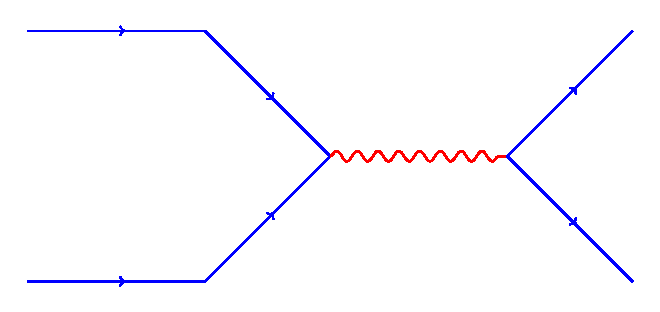
\includegraphics[width=0.8\textwidth]{w_production}
  \caption{Diagram of a W boson production and leptonic decay at a hadron-hadron collider.}
  \label{wbos:wproddiag}
\end{figure}

At proton-proton colliders the \PW production cross section is given by the
convolution of the cross section at the parton level, and the parton
distribution functions (PDF) of the protons,
\begin{multline}
  d\sigma_{(\HepProcess{h_1 h_2 \to \PWpm})}(p_1,p_2;Q^{2}) = \\
  \sum\limits_{a,b}
  \int_0^1 \! \mathrm{d} x_1 
  \int_0^1 \! \mathrm{d} x_2 
  f_a^{h_1}(x_1,Q^2)
  f_b^{h_2}(x_2,Q^2) 
  d\hat{\sigma}_{(\HepProcess{a b \to \PWpm})}(x_1 p_1, x_2 p_2; Q^2),
  \label{wbos:xsec}
\end{multline}
where $\sum\limits_{a,b}$ represents the sum over the initial parton states $a$
and $b$, $f_a^{h}(x,Q^2)$ represents the proton {PDF} and
$d\hat{\sigma}_{(\HepProcess{a b \to \PWpm})}(x_1 p_1, x_2 p_2; Q^2)$
represents the partonic sub-process cross section.

\subsubsection*{Partonic Sub-Process}

At {LO} the process for a \PWp is
\begin{equation}
  \HepProcess{\Pup + \APdown \to \PWp \to \Pleptonplus \Pnulepton} 
  \label{wbos:wpprod} 
\end{equation}
and for a \PWm:
\begin{equation}
  \HepProcess{\APup + \Pdown \to \PWm \to \Pleptonminus \APnulepton}
  \label{wbos:wmprod} 
\end{equation}

\begin{figure}[htbp]
  \centering
  \begin{subfigure}{0.45\textwidth}
    \centering
    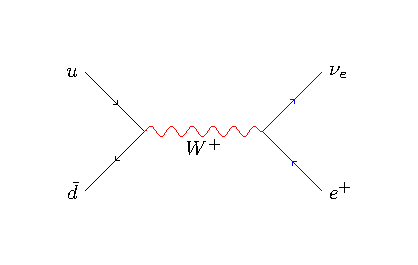
\includegraphics[width=\textwidth]{w_process_wp}
    \caption{\HepProcess{\Pup + \APdown \to \PWp \to \Pleptonplus \Pnulepton}}
    \label{fig:w_process_wp}
  \end{subfigure}
  \begin{subfigure}{0.45\textwidth}
    \centering
    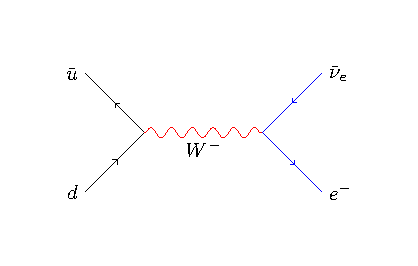
\includegraphics[width=\textwidth]{w_process_wm}
    \caption{\HepProcess{\APup + \Pdown \to \PWm \to \Pleptonminus \APnulepton}}
    \label{fig:w_process_wm}
  \end{subfigure}
  \caption{Tree-level diagrams for \PWp and \PWm boson production and electron
decay at a hadron-hadron collider.}\label{fig:w_process} 
\end{figure}

Tree-level Feynman diagrams representing these processes are shown in
\FigureRef{fig:w_process}.
At the {LHC} (a proton-proton collider), one parton is most to likely be a
valence quark with a high fraction of the proton's momentum, and the other
parton will tend to be a sea anti-quark with a lower fraction of the momentum
than the quark. The difference in momentum of the partons causes the \PW bosons 
to tend to be produced at higher rapidities. 

\subsubsection*{Proton Parton Distribution Function} 
The proton parton distribution function (PDF) represents the number density of
parton $a$ that has a momentum fraction $x+\mathrm{d}x$ of the colliding hadron
$h$.  

\begin{figure}[htbp]
  \centering
  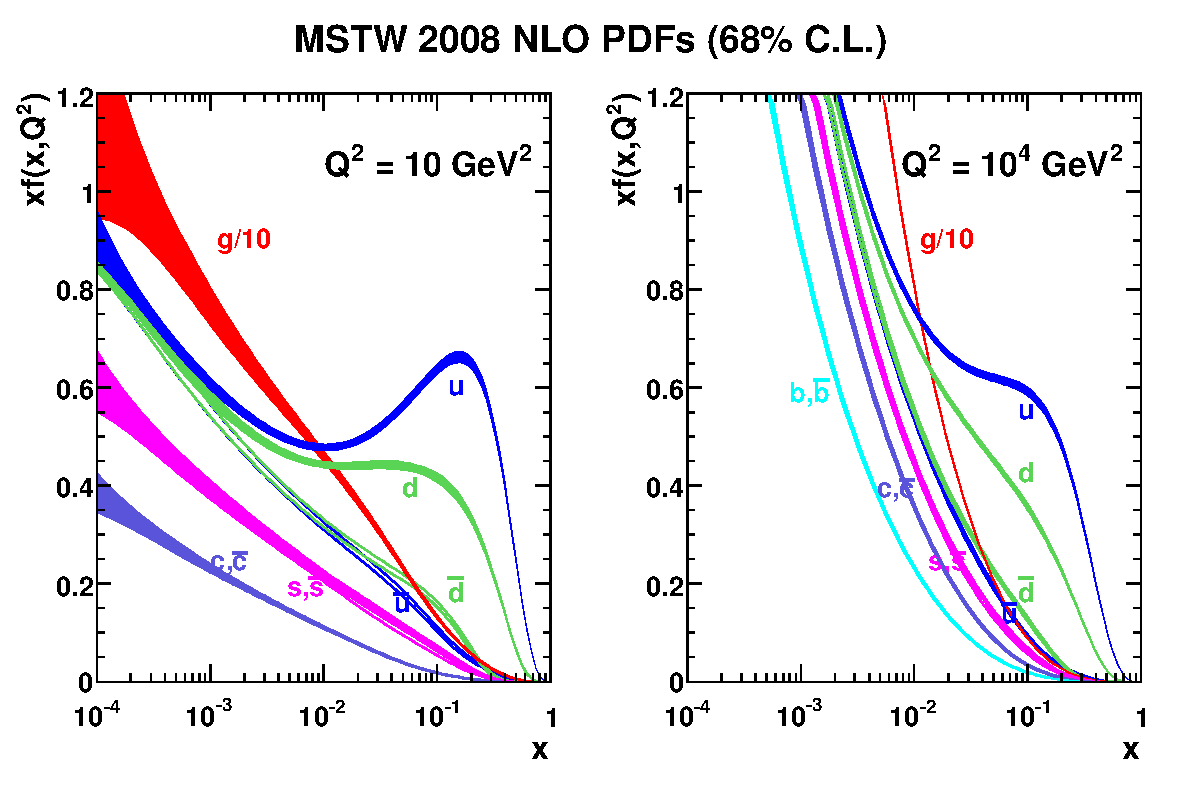
\includegraphics[width=\textwidth]{mstw2008nlo68cl_allpdfs}
  \caption[Proton PDF at  $ Q^2 = \unit{ 10  }{\GeV^2} $ and $ Q^2 = \unit{ 100
}{\GeV^2} $.] {Proton PDF at  $ Q^2 = \unit{ 10  }{\GeV^2} $ (left) and $ Q^2 =
\unit{ 100  }{\GeV^2} $ (right) from \cite{martin2009parton}.}
  \label{wbos:pdf}
\end{figure}

The {PDFs} are obtained from global fits to experimental data
\cite{martin2009parton}.  \FigureRef{wbos:pdf} (right) shows the proton PDF at
$Q^2\approx M_{\PW}^2$ from the MSTW group.  The anti-quark parton densities
$\APup(x,Q^2)$ and $\APdown(x,Q^2)$ are relatively similar especially at the LHC
energies, where the parton momentum fraction, x, tends to be small.
However, the {PDF} for the valence quarks in the proton differ, 
the up-type quark dominates over the down-type quark.
This is due to the excess of up-type valence quarks with respect to down-type
valence quarks in the proton (\HepProcess{\Pup\Pup\Pdown}). 
This can be seen in the ratio of the up-type and the down-type {PDFs},
\begin{equation}
  R_{ud}(x,Q^2) = \frac{\Pup(x,Q^2)}{ \Pdown(x,Q^2)} > 1,
\end{equation}
where $\Pup(x,Q^2)$ are the up and down quark {PDFs}.
\FigureRef{fig:pdf_plots} shows the ratio of the up-type and down-type
quarks.  The ratio $R$ changes as a function of $x$, $R \approx 1$ for $x \ll 1$
and increases monotonically as $x$ increases.  The up-type quark will have a
greater fraction of the proton's momentum than the down-type quark.

\begin{figure}[htbp]
  \centering
  %\begin{subfigure}{\textwidth}
    %\centering
    %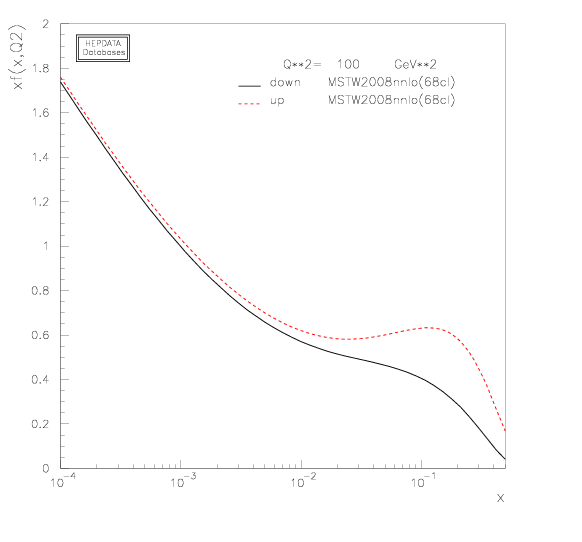
\includegraphics[width=0.75\textwidth]{plot_pdf}
    %\caption{PDF for \Pup and \Pdown}
    %\label{fig:plot_pdf}
  %\end{subfigure}
  %\begin{subfigure}{\textwidth}
    %\centering
    %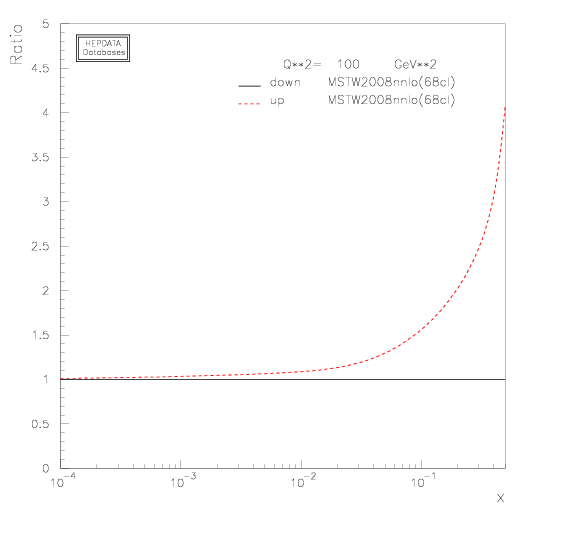
\includegraphics[width=0.75\textwidth]{plot_pdf_ratio}
    %\caption{Ratio for \Pup and \Pdown PDF}
    %\label{fig:plot_pdf_ratio}
  %\end{subfigure}
  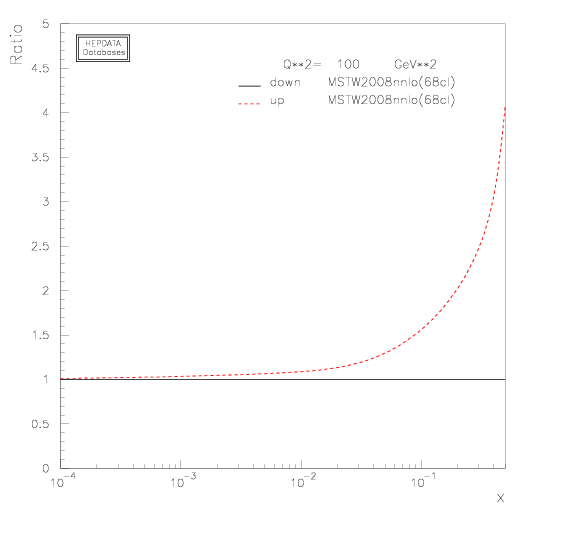
\includegraphics[width=0.75\textwidth]{plot_pdf_ratio}
  \caption[Ratio of up quarks to down quarks, $R_{ud}$ at
$Q^2=\unit{100}{\GeV^2}$.] {Ratio of up quarks to down quarks, $R_{ud}$ at
$Q^2=\unit{100}{\GeV^2}$.  Generated from \cite{hepdata} using the MSTW200nlo
PDFs \cite{martin2009parton}.}
  \label{fig:pdf_plots} 
\end{figure}

\subsection{\PW Boson Rapidity Distribution}
\label{wbos:wrapsec}

The rapidity of a particle is defined in \EquationRef{eq:rapidity}.  It
represents the boost along the beam axis required to go from the lab frame to
the frame where the particle is produced perpendicular to the beam axis.

\begin{figure}[htbp]
  \centering
  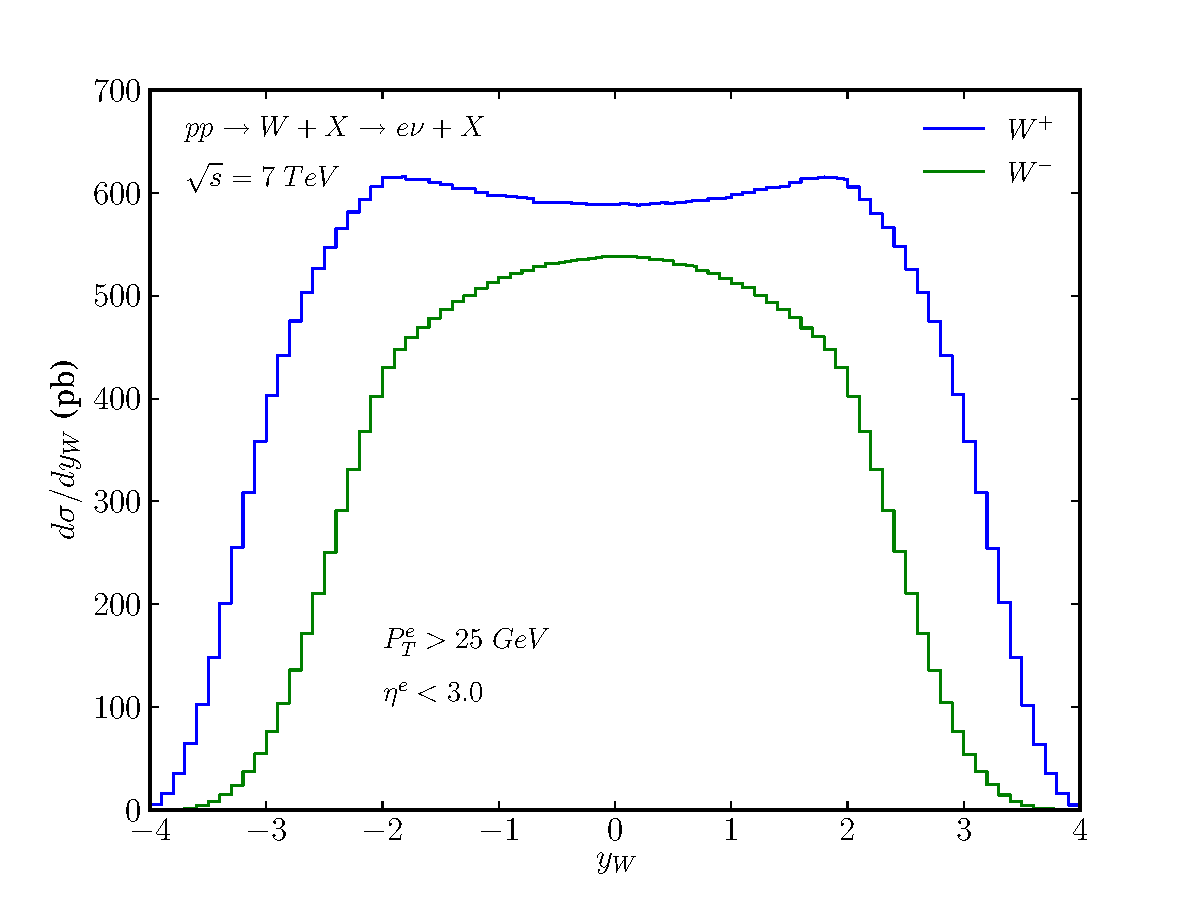
\includegraphics[width=0.8\textwidth]{w-rapidity}
  \caption[The rapidity distribution for \PWp and \PWm at the LHC
$\sqrtS=\unit{7}{\TeV}$ proton-proton collisions.] {The rapidity distribution
for \PWp and \PWm at the LHC $\sqrtS=\unit{7}{\TeV}$ proton-proton collisions.
Generated with the MSTW2008nlo PDF\cite{martin2009parton} interfaced with the
MCFM generator tool \cite{campbellmcfm}.}
  \label{wbos:wrapid}
\end{figure}

The rapidity distributions, $y_W$, for \PWp and \PWm bosons produced at the
{LHC} are shown in \FigureRef{wbos:wrapid}.  The \PWp cross section is greater
than the \PWm cross section.  This is a consequence of the different production
processes for \PWp and \PWm (shown in \EquationRef{wbos:wpprod} and
\EquationRef{wbos:wmprod} respectivly) and the {PDF} for the valence quarks in
the proton differing as seen in \FigureRef{fig:pdf_plots}. The up-type quark
{PDF} dominates over the down-type which leads to a greater \PWp production rate
than \PWm.

It is also seen in \FigureRef{wbos:wrapid} that the \PWm tends to be produced
more centrally whereas the \PWp can be produced at larger rapidities. This is due
to up-type quarks tending to carry a greater fraction of the proton's momentum,
$x$, than the down-type quarks as seen in \FigureRef{fig:pdf_plots}.

The momentum fraction, $x$, of the interaction quarks is correlated with the
rapidity of the \PW boson. Therefore, the ratio of $\Pup$ and $\Pdown$ quarks as
a function of momentum fraction, $x$, is directly related to the difference in
cross sections for \PWp and \PWm production as a function of the boson rapidity.

Therefore a measurement of the asymmetric production of \PW bosons, as a
function of the rapidity of the boson, at the {LHC} provides important
information on the ratio of the up-type and down-type quark parton densities as
a function of $x$,
$R_{ud}(x,Q^2)$, within the proton\cite{kom}. 

\subsection{\PW Boson Charge Asymmetry}

The \PWpm boson charge asymmetry is defined as,
\begin{equation}
  A_{W}(y_{\PW})=
    \frac{ 
      \nicefrac{ d\sigma (\PWp) }{ dy_{W} } -
      \nicefrac{ d\sigma (\PWm) }{ dy_{W} }
    }
    {
      \nicefrac{ d\sigma (\PWp) }{ dy_{W} } +
      \nicefrac{ d\sigma (\PWm) }{ dy_{W} }
    }
,
\label{wbos:wasym}
\end{equation} 
where $y_{W}$ is the boson rapidity, and 
$\nicefrac{ d\sigma (\PWpm) }{ dy_{W} }$ is the \PWpm production cross section
at a fixed $y_{W}$.  
If $d\sigma(\PWp) > d\sigma(\PWm) $ then $A_{W}(y_{\PW})> 0$,
else if $d\sigma(\PWp) < d\sigma(\PWm) $ then $A_{W}(y_{\PW})< 0$,
and for symmetric \PWpm boson production, $A_{W}(y_{\PW})= 0$,

The prediction for the W boson charge asymmetry as a function of the boson
rapidity is shown in \FigureRef{wbos:chargeasym}. $A_{W}(y_{\PW})> 0$ and
increases as the rapidity increases.

\begin{figure}[htbp]
  \centering
  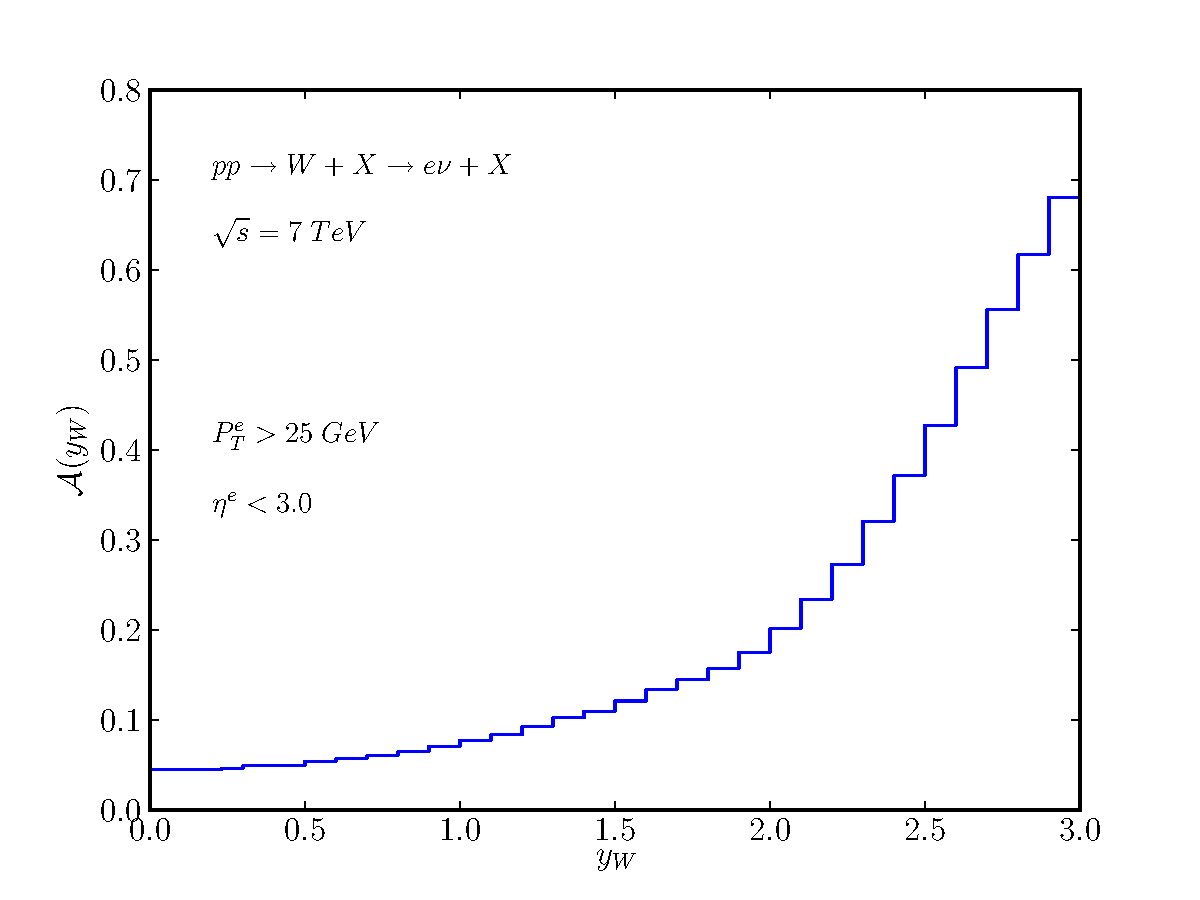
\includegraphics[width=0.8\textwidth]{w-asym}
  \caption[\PW boson charge asymmetry at LHC in $\sqrtS=\unit{7}{\TeV}$
proton-proton collisions.] {\PW boson charge asymmetry at LHC in
$\sqrtS=\unit{7}{\TeV}$ proton-proton collisions.  Generated with the
MSTW2008nlo PDF\cite{martin2009parton} interfaced with the and the MCFM
generator tool \cite{campbellmcfm}.}
  \label{wbos:chargeasym}
\end{figure}

\PW bosons are identified by their decay to a lepton plus neutrino, however at
hadronic colliders the neutrino longitudinal momentum cannot be determined
which means that the \PW rapidity, $y_{W}$, cannot be measured.  Instead what
is studied is the charge asymmetry in the leptons that result from the \PW boson
decaying leptonically.

%It is possible to overcome the difficulty in determining the boson rapidity
%by extrapolating the neutrino longditudinal momentum from the lepton neutrino
%with a {MC} study. 

\section{W Boson Decay}
The \PW boson will decay to either a lepton and neutrino, or a pair of up and
down quarks. The branching fractions for the various decays are shown in
\TableRef{tab:w_decay}.
This thesis will consider the electron decay of the \PW boson which will occur
in approximately $11\%$ of \PW decays.

\begin{table}[htbp]
\begin{center}
\begin{tabular}{l l }
\toprule
\PWp Decay Mode & Fraction ($\Gamma_{i}/\Gamma$)\% \\
\midrule
\APelectron\Pnu & $10.75\pm0.13$ \\
\APmuon\Pnu     & $10.57\pm0.15$ \\
\APtauon\Pnu    & $11.25\pm0.20$ \\
hadrons         & $67.60\pm0.27$ \\
\bottomrule
\end{tabular}
\caption[Experimentally measured \PWp decay modes.] {Experimentally measured
\PWp decay modes. The decay modes of \PWm are the charge conjugates of the \PWp.
From \cite{beringer2012review}.\label{tab:w_decay}} 
\end{center}
\end{table}

\subsection{Electron Pseudorapidity Distribution}
The rapidity distributions of the charged leptons produced from \PWpm decay are
further complicated by the charge asymmetric decay of the \PWpm boson. 
The asymmetric decay arises due to the $V-A$ coupling of the \PW boson to the
annihilating \HepProcess{\Pquark\APquark} pair and the decaying lepton pair.

At leading order (LO) the \PWp is produced in the annihilation of a \Pup valance quark
with a \APdown sea-quark (\EquationRef{wbos:wpprod}). 
If the parton masses, are neglected the \Pup is left-handed and the \APdown is
right-handed, as shown at the top of \FigureRef{wbos:wspin}. 

In the \PWp decay the \Ppositron is right-handed and the \Pnue is left-handed.
\FigureRef{wbos:wspin} shows that if the  positron is produced in the same direction
as the incoming \APdown quark angular momentum is conserved and the decay is
allowed.
However the decay where the positron is produced in the same direction as the
incoming \Pup quark is forbidden.
A similar argument holds true for \PWm decays, where the \Pelectron is produced
preferentially in the direction of the \Pdown quark.

\begin{figure}[htbp]
  \centering
  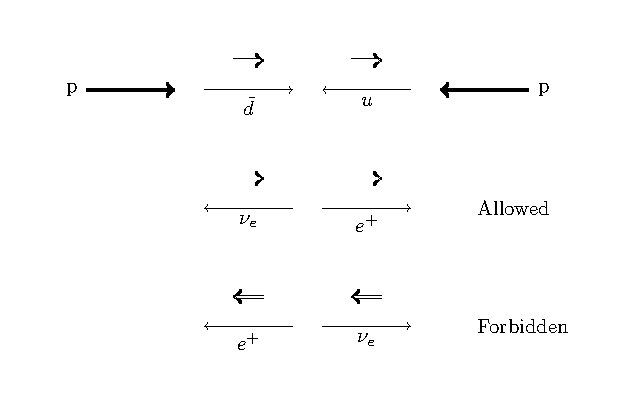
\includegraphics[width=0.8\textwidth]{w_decay_directions}
  \caption[Preferred directions of electron spins in
\HepProcess{\PWplus\to\APelectron\Pnue} decay.] {Preferred directions of
electron spins in \HepProcess{\PWplus\to\APelectron\Pnue} decay.  The heavy
arrows show the directions of the incoming protons, the thin arrows show the
directions of the incoming quarks and the outgoing electron and neutrino. The
double arrows show the spins.  Modified from \cite{aitchison2004gauge}. }
  \label{wbos:wspin}
\end{figure}

The distribution of the electron from \PWpm decay in the massless limit
is given by\cite{perkins2000introduction,aitchison2004gauge},
\begin{equation}
  \frac{1}{\sigma_{u\bar{d}}}
  \frac{d \sigma_{u\bar{d}}}{d \cos \theta_{\Plepton d}^{\ast}}
  =
  \frac{1}{\sigma_{d\bar{u}}}
  \frac{d \sigma_{d\bar{u}}}{d \cos \theta_{\Plepton d}^{\ast}}
  \propto
  (1+\cos \theta_{\Plepton d}^{\ast})^2
  \label{wbos:lepton}
\end{equation}
where $\theta_{\Plepton d}^{\ast}$ is the scattering angle of the charged
lepton with respect to the direction of the down-type quark or anti-quark, in
the centre of mass system of the two quarks. The cross section is maximised when
$\theta_{\Plepton D}^{\ast}$ is minimised and the charged lepton is produced in
the same direction as the down-type quark.

The rapidity distribution of the electron is therefore a convolution of the
{electroweak} correlations in \EquationRef{wbos:lepton} with the \PW rapidity
described in \SectionRef{wbos:wrapsec}.  In proton-proton collisions the \PWp
tends to be produced in the direction of the \Pup.  However, due to the
electroweak correlations the charged lepton from the decaying \PWp will tend to
be produced along the direction of the down-type quark and therefore will shift
the rapidity distribution of the lepton to be more central. Similarly, \PWm
bosons tend to be produced more centrally, however the electroweak correlations
will shift the charge lepton rapidity distribution to higher rapidities.

\FigureRef{fig:leptonrapidity} shows the Monte Carlo (MC) generated
pseudorapidity distribution of electrons and positrons produced in
$\sqrtS=\unit{7}{\TeV}$ proton-proton collisions.  The pseudorapidity is defined
in \EquationRef{eq:pseudorapidity}. In the massless approximation, the
pseudorapidity of the electron is equal to the rapidity.

\todo{e+ and e- PT distributions?}
\todo{$\eta$ or $\eta_e$}

\begin{figure}[htbp]
  \centering
  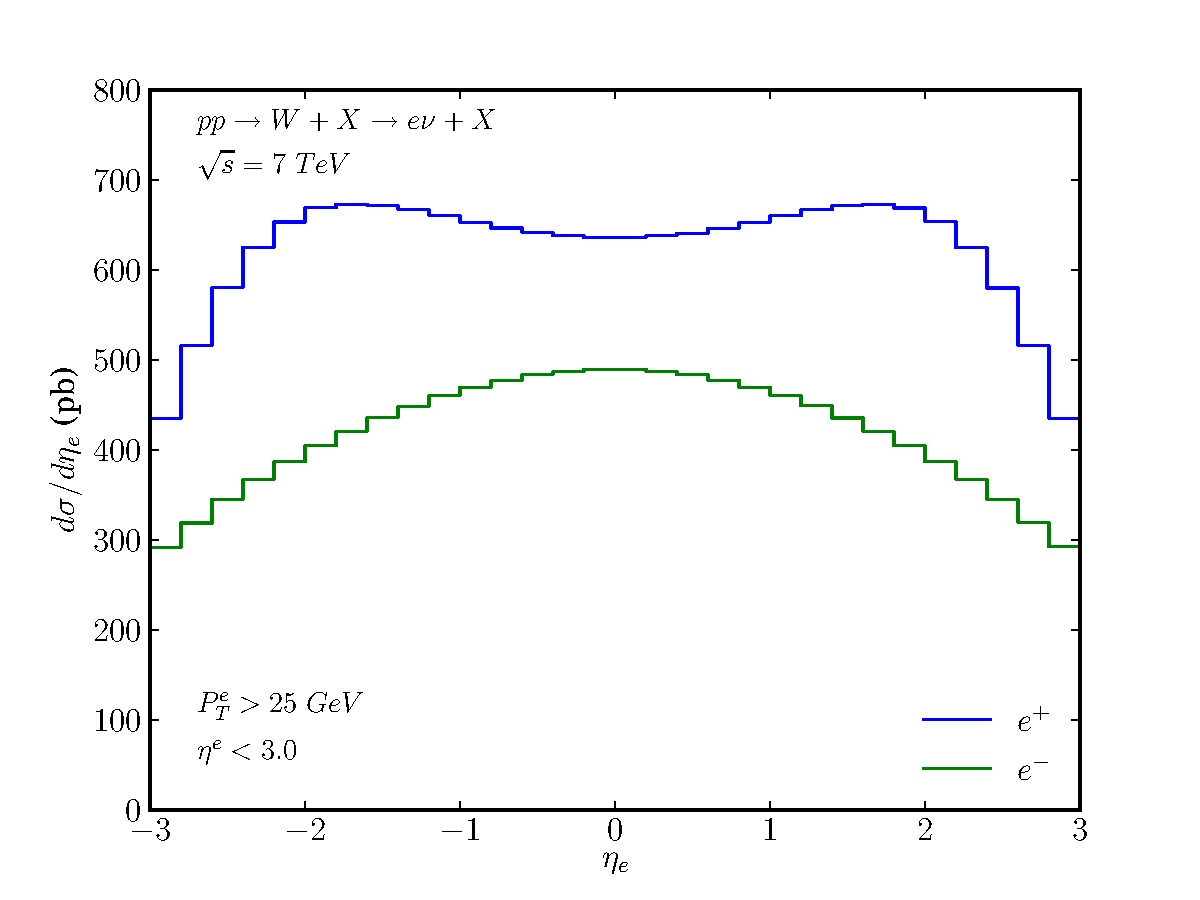
\includegraphics[width=0.8\textwidth]{lepton-rapidity}
  \caption[Electron and positron pseudorapidity, $\eta_e$, distributions in
$\sqrtS=\unit{7}{\TeV}$ proton-proton collisions.] {Electron and positron
pseudorapidity, $\eta_e$, distributions in $\sqrtS=\unit{7}{\TeV}$ proton-proton
collisions.  Generated with the MSTW2008nlo PDF\cite{martin2009parton}
interfaced with the MCFM generator tool \cite{campbellmcfm}.}
  \label{fig:leptonrapidity}
\end{figure}

\subsection{Electron Charge Asymmetry}

The electron asymmetry is defined in \EquationRef{eq:AsymThe} analogously to the
\PW boson asymmetry in \EquationRef{wbos:wasym}, as the difference in the
\HepProcess{\PWplus \to \APelectron} and \HepProcess{\PWminus \to \Pelectron}
over the total \inclusiveWe cross section.
\begin{equation}
A_{the}(\eta)=\frac{  \frac{d\sigma}{d\eta}(\Wpenu) -
\frac{d\sigma}{d\eta}(\Wmenu) }{ \frac{d\sigma}{d\eta}(\Wpenu) +
\frac{d\sigma}{d\eta}(\Wmenu) }
\label{eq:AsymThe}
\end{equation} 

The electron charge asymmetry has previously been studied in $p\bar{p}$
collisions by the CDF and D0 experiments at the Fermilab Tevatron collider
\cite{cdfWAsym,d0WAsym}. 

\FigureRef{wbos:asym_simple} shows the electron charge asymmetry prediction for
electron transverse momentum cuts of \unit{25}{\GeV}. The prediction was
produced using the MSTW2008NLO PDF\cite{martin2009parton} set.
Unlike the \PW asymmetry, the electron asymmetry turns over at $\eta\approx
2.25$. This effect is due to the electroweak correlations in the leptonic decay of
the \PW boson.

\begin{figure}[htbp]
  \centering
  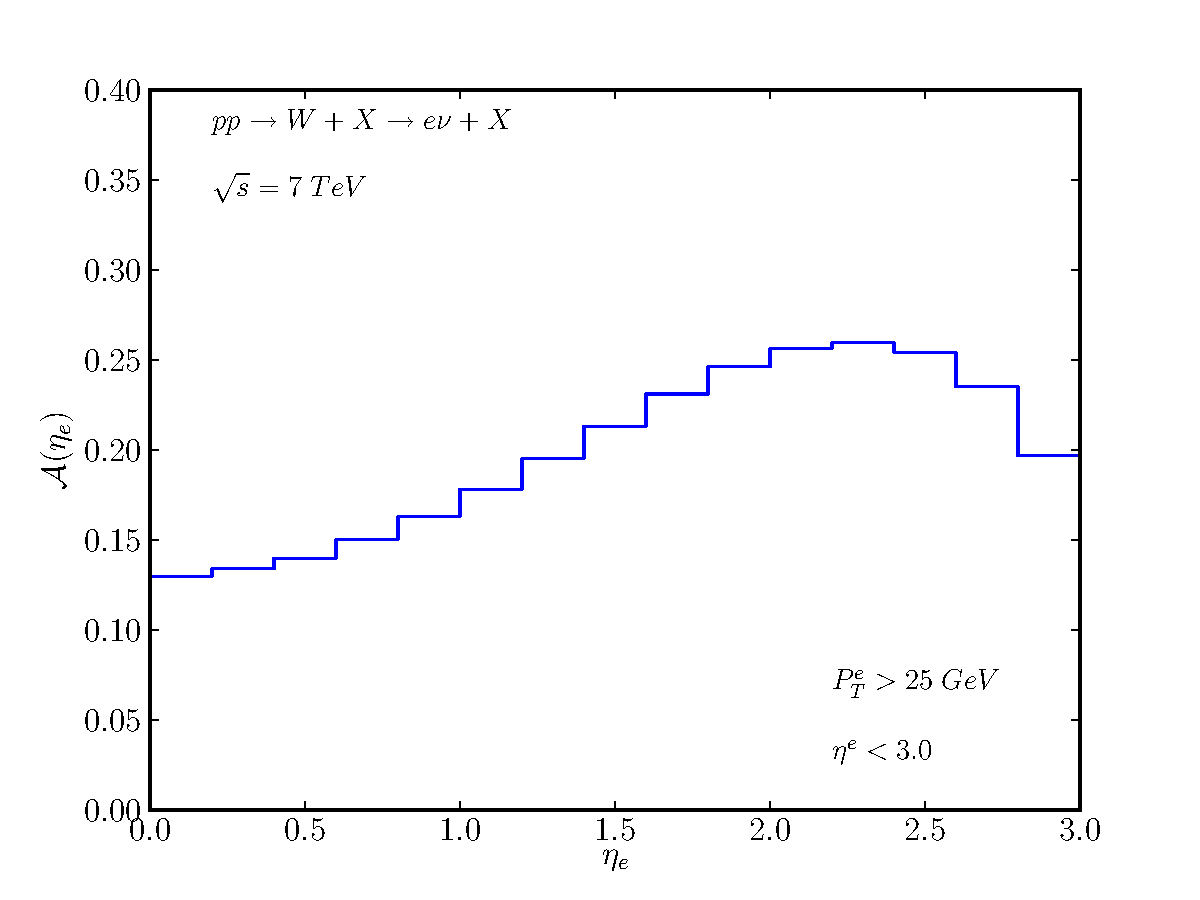
\includegraphics[width=0.8\textwidth]{lepton-asym}
  \caption[Electron charge asymmetry at LHC in $\sqrtS=\unit{7}{\TeV}$
proton-proton collisions.] {Electron charge asymmetry at LHC in
$\sqrtS=\unit{7}{\TeV}$ proton-proton collisions.  Generated with the
MSTW2008nlo PDF\cite{martin2009parton} interfaced with the MCFM generator tool
\cite{campbellmcfm}.}
  \label{wbos:asym_simple}
\end{figure}

In an experiment, the cross section is not measured directly, instead what is
measured are the electron and positron yields.  The experimentally measured
asymmetry is given by \EquationRef{eq:AsymExp},
\begin{equation}
A_{exp}(\eta)=\frac{  \frac{dN}{d\eta}(\Pelectron) -
\frac{dN}{d\eta}(\APelectron) }{ \frac{dN}{d\eta}(\Pelectron) +
\frac{dN}{d\eta}(\APelectron) }
\label{eq:AsymExp}
\end{equation} 

To get from the experimentally measured asymmetry to the lepton charge
asymmetry, \EquationRef{eq:NumEve} must be used, which takes into
account the experimental effects such as the luminosity (${\cal L}$), high
level trigger ($\epsilon_{HLT}$), offline efficiency ($ \epsilon_{off}$) and
the acceptance ($\epsilon_{acc}$).

\begin{equation}
\frac{dN}{d\eta} = {\cal L } \frac{d\sigma}{d\eta}  \epsilon_{HLT}
\epsilon_{off} \epsilon_{acc}
\label{eq:NumEve}
\end{equation} 
As the asymmetry is a ratio, the luminosity, high level trigger and the
offline efficiency can be cancelled out assuming that they are not asymmetric
with respect to charge. 

The acceptance cannot be cancelled, it is a function of transverse momentum of
the electron, and these distributions will differ for \Pelectron and \APelectron.
A correction due to acceptance effect could be included, but would be highly
dependent on the choice of PDF used to generate the corrections \cite{cdfWAsym}.
The measurements presented in this thesis do not correct for acceptance effects.

%\begin{align} 
%A_{exp}(\eta) &= \frac{ \frac{dN}{d\eta}(\Pelectron) -
%\frac{dN}{d\eta}(\APelectron) }{ \frac{dN}{d\eta}(\Pelectron) +
%\frac{dN}{d\eta}(\APelectron) }\\   
              %&= \frac{ \frac{d\sigma}{d\eta}(\Wpenu) -
%\frac{\epsilon^{-}_{acc}}{\epsilon^{+}_{acc}} \frac{d\sigma}{d\eta}(\Wmenu) }{
%\frac{d\sigma}{d\eta}(\Wpenu) + \frac{\epsilon^{-}_{acc}}{\epsilon^{+}_{acc}}
%\frac{d\sigma}{d\eta}(\Wmenu) }
%\label{eq:AsymExpCorr}
%\end{align}

\section{Electron Charge Asymmetry Theoretical Predictions}
\label{sec:asymuncert}

In this section predictions for the electron charge asymmetry are investigated in
detail.  The predictions are calculated using MCFM\cite{campbellmcfm} {MC} tools
interfaced with the LHAPDF package\cite{whalley2005houches}.  LHAPDF provides an
interface to many different {PDF} sets. For the following predictions, PDFs from
the MSTW \cite{martin2009parton} and CTEQ \cite{lai2010vv} collaborations are
used.

\subsection{Uncertainty on Theoretical Predictions}
The theoretical predictions of the electron charge asymmetry will have an error
associated with the uncertainty on the {PDF}.
The uncertainty on the {PDF} originates from the experimental errors on the
data used in the global fits performed by each of the {PDF} collaborations.



Each {PDF} collaboration produces a set of {PDFs} that include the
central value, or best fit to experimental data, and $2N$ error {PDFs}, where
$N$ is the number of free parameters used in the global
fit\cite{Bourilkov:2006cj}.
For each of the free parameters there is a PDF produced with the parameter at its upper
error and another with the parameter at its lower error. 

The uncertainty on the observable, in this case the lepton asymmetry, is found
by producing $2N+1$ theoretical predictions, one for each member of the {PDF}
set. The predictions are then used to approximate the {PDF} uncertainty by
using the `master equation'\cite{Bourilkov:2006cj,campbell2006hard}.
For the upper uncertainty,

\begin{equation}
\Delta A^{+}_{max}
= \sqrt{ \sum^{N}_{i=1} \left[ max( A^{+}_i-A_{0}, A^{-}_i-A_{0}, 0 ) \right]^{2}}
\end{equation}
and for the lower uncertainty,
\begin{equation}
\Delta A^{-}_{max}
= \sqrt{ \sum^{N}_{i=1} \left[ max( A_{0}-A^{+}_i, A_{0}-A^{-}_i, 0 ) \right]^{2}}
\end{equation}
where $A^{\pm}_{i}$ is the asymmetry prediction using the {PDF} with the
positive/negative fluctuation of parameter $i$ and $A_{0}$ is the prediction
using the central value.

\subsection{Prediction of the Electron Charge Asymmetry above \unit{25}{\GeV}}

\begin{figure}[htbp]
  \centering
  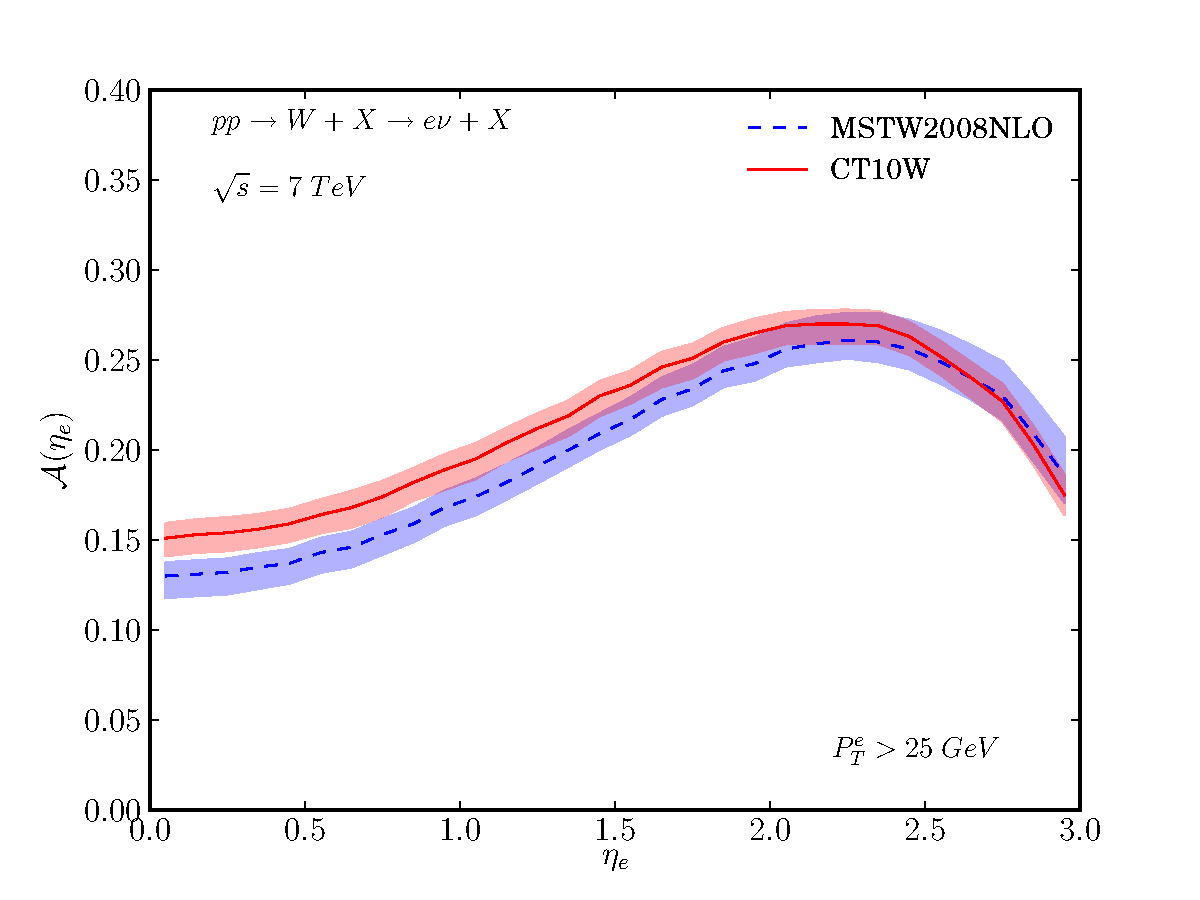
\includegraphics[width=0.8\textwidth]{asym-uncert}
  \caption[The theoretical electron charge asymmetry for a $\pT>\unit{25}{\GeV}$
with the {PDF} uncertainties.] {The theoretical electron charge
asymmetry\cite{monchenault2011predictions} for a $\pT>\unit{25}{\GeV}$ with the
{PDF} uncertainties for the {PDF} sets MSTW08NLO\cite{martin2009parton} and
CT10W\cite{lai2010vv}. The uncertainties are $68\%$ confidence level. The
predictions are generated using the {MCFM} \cite{campbellmcfm} generator.}
  \label{fig:asym-uncert}
\end{figure}

\FigureRef{fig:asym-uncert} shows the theoretical predictions for the electron charge asymmetry 
for $\pT>\unit{25}{\GeV}$ with PDFs
from the MSTW collaboration\cite{martin2009parton} and the CTEQ collaboration\cite{lai2010vv}.
The uncertainty due to the PDFs is included.
The predictions show a disagreement with the asymmetry at low rapidities. The
CTEQ tends to be higher and the MSTW lower. The disagreement is greater than the
PDF uncertainty on the measurement.

\subsection{Prediction of the Electron Charge Asymmetry above \unit{30}{\GeV}}

\begin{figure}[htbp]
  \centering
  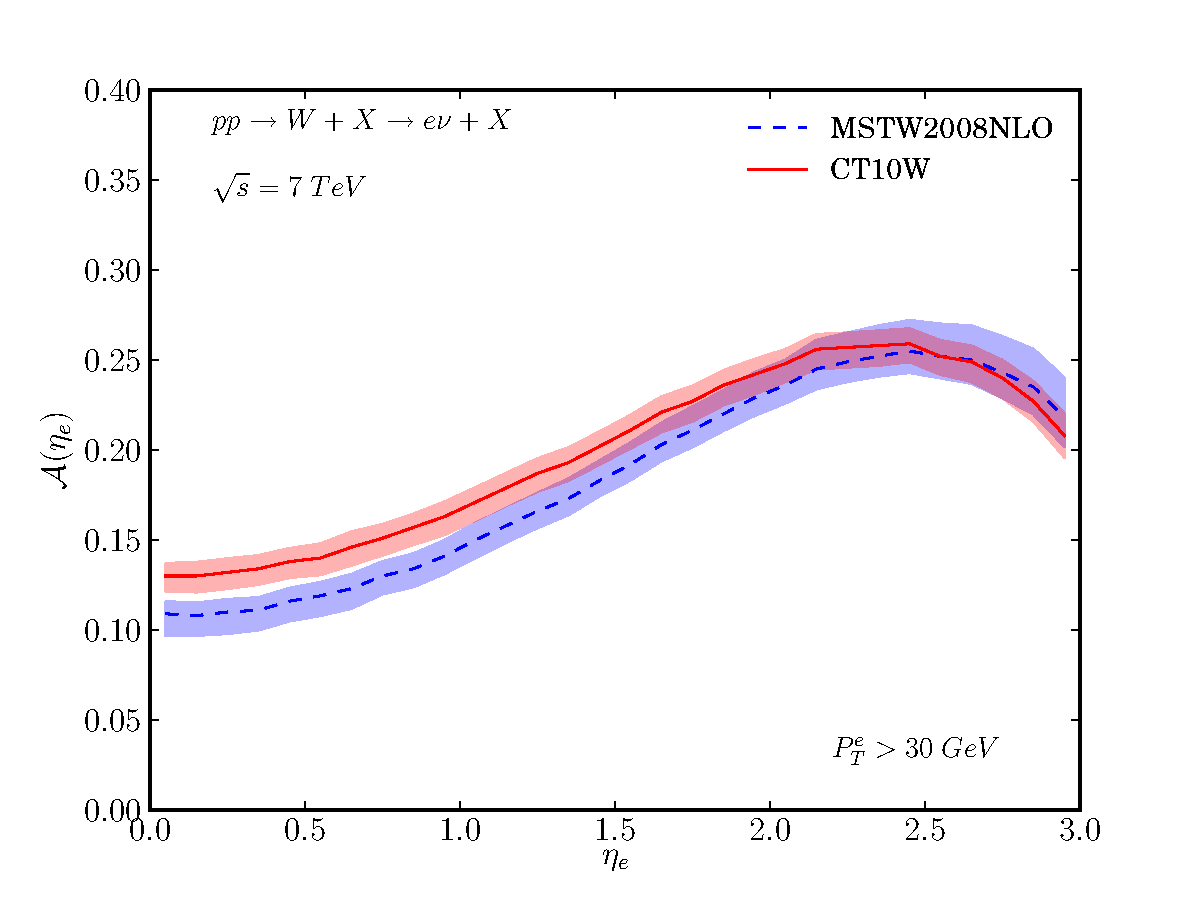
\includegraphics[width=0.8\textwidth]{asym-uncert-30}
  \caption[The theoretical electron charge asymmetry for a $\pT>\unit{25}{\GeV}$
with the {PDF} uncertainties.] {The theoretical electron charge
asymmetry\cite{monchenault2011predictions} for a $\pT>\unit{30}{\GeV}$ with the
{PDF} uncertainties for the {PDF} sets MSTW08NLO\cite{martin2009parton} and
CT10W\cite{lai2010vv}. The uncertainties are $68\%$ confidence level. The
predictions are generated using the {MCFM} \cite{campbellmcfm} generator.}
  \label{fig:asym-uncert-30}
\end{figure}

\FigureRef{fig:asym-uncert-30} shows the theoretical predictions for the electron charge asymmetry 
for $\pT>\unit{30}{\GeV}$ with PDFs
from the MSTW collaboration\cite{martin2009parton} and the CTEQ
collaboration\cite{lai2010vv}.  Similar disagreement between the asymmetry
predictions at low rapidities is seen.

The asymmetry prediction at low rapidities is lower than the prediction with an
electron cut at \unit{25}{\GeV}. The turning point in the asymmetry is also
shifted to higher rapidities.


